\section{Problem Framing}
\label{s:prob_frame}
\subsection{Introduction}
Through the years, the river IJssel has been of incredible importance in Dutch history. In times of prosperity the river was trading route, in times of war it made up a strategically defendable border. Situated along this river, between the two bigger cities of Deventer and Zutphen, one can find the smaller town of Gorssel. Located along the banks of the IJssel river, water management and flood prevention have both been interwoven with the town's existence since the first farmers situated themselves there. However, when in 1993 and 1995 the water rose to dangerous levels in the IJssel, the discussion on water management became a national interest and thus, the Room for the River initiative was born. (\textbf{Cite Rijke et al.}) However, the fight against water continues. With global warming added into the mix, the rivers currently face even greater pressure (\textbf{Cite Takken}) and a waterproof water protection plan is key for the future of Gorssel and its farmers. Besides the complexity such a plan inherently has, this particular problem requires a careful examination of the actor field, for there are many involved stakeholders. It can fairly be assumed that all parties want to prevent a life-threatening flood, but beneath that, all involved parties have their own objectives they aim to achieve.  

This report uses innovative modelling and analysis techniques to analyse options for the planning of flood protection measures along the IJssel river. As explained, the problem of flood management in this region is complex, due to significant uncertainties (i.e. flood wave shapes, dike failure probabilities, and breach widths) and conflicting priorities of different stakeholders in the region. Here, exploratory modelling and analysis is used to support decision making under the deep uncertainty this complexity causes. This model-based decision making is performed from the perspective of our problem owner, Gorssel, in addition to two key stakeholders of interest: Overijssel Regional Government and the city of Deventer. This is done to reveal important trade-offs and the outcomes of conflicting objectives to inform the policy-making process in the Overijssel region.

%\textcolor{red}{1-2 sentences on categorisation of this as a complex problem. what level of uncertainty is it (see intro to Marchau book)? Why do we need to use DMDU techniques?}
% I wasn't completely in agreement with this but that might be my take

% Problem framing; the decision problem can be structured in many ways. 
% Our problem owner is Gorssel


\subsection{Research question}

%What do you see as the key objectives and constraints?
Protecting the livelihoods of those that reside in Gorssel is Gorssel's main objective. Their residents mostly comprise of farmers and so their livelihood consists the crops they organically grow. Gorssel wants to minimise flood risk and expected flood damage but also prevent land encroachment to preserve the amount of land available for farming. Both of these are not favourable but are currently in a trade-off with each other. However, there is a limit to how much land Gorssel wants encroached upon - too much, and the farmers are left without anything. Furthermore, it is also important that Gorssel is not treated lesser than the surrounding cities and that everyone is treated in a "fair" way. 
The goal of this report is to find a strategy for Gorssel to navigate these difficult waters. 

% I'm not sure how explicitly to discuss the constraints 

%How are you framing the problem? 
The research question that is in line with this goal is as follows: 
\begin{quote}
    How can Gorssel (Dike Ring 4) affordably protect it's citizens and businesses from flood risk to a similar level as neighbouring urban areas, while still preserving and protecting farmland from encroachment?
\end{quote}

This question was informed by the mandate for Gorssel provided as part of the EPA1361 Debate (see Chapter \ref{s:poli_reflect} for more information), in addition to formal documentation of the Room for the River project, conducted by Rijkswaterstaat between 2010 and 2019 (CITE: Rijkswaterstaat).

To explore suitable policies for achieving these objectives, a problem formulation in the EMA Workbench was devised.
The prioritised objectives for the Gorssel-perspective problem formulation are:
\begin{itemize}
    \item Minimise Expected Annual Damage for Gorssel: This objective reflects Gorssel's desire to generally minimise flood risk, while also reflecting effects of damage to farms and other property
    \item Minimise Expected Number of Deaths for Gorssel: This objective reflects Gorssel's desire to generally minimse flood risk.
    \item Minimise Total Costs: This objective reflects the desire to reduce the cost impact of flood mitigation measures taken across the entire IJssel River system. Total costs for all actors was considered relevant given the requirement of cost sharing for flood mitigation activities across the region.
    \item Difference in Expected Annual Damage (EAD) between Gorssel and Deventer (information only - no objective set): This function returns results on the difference in Expected Annual Damages between Gorssel and Deventer, but will not be optimised for. The results for this feature under different policies serves to provide information on the relative 'fairness' in terms of rural-urban burden sharing in terms of flood risk, and as an additional feature for informing satisficing or regret-based robustness metrics.
    \item Difference in Expected Number of Deaths between Gorssel and Deventer (information only - no objective set): rationale for inclusion of this metric is as for difference in EAD.
\end{itemize}
These five core objectives are a refinement of all available objectives. These were prioritised due to the computational limitations of the exploratory modelling and analysis approaches (as explained in Section \ref{s:approach}) and due to limitations in stakeholder comprehension of multiple objectives. As a we have chosen not to present the analysis in the format of dynamic adaptive policy pathways, all objective outcomes were aggregated to a single planning step. 
%What levers are relevant, and what is being treated as uncertain.
For Gorssel, the relevant levers were:
\begin{itemize}
    \item Dike Ring: Gorssel has the option to switch on and off the 
    \item Early Warning System: Applied across the whole region
    \item Room for the River: Applied across the whole region
\end{itemize}

\subsection{Actor Analysis}
%Which other actors are we analysing and why are they natural coalition partners for Gorssel?
The basic analysis of preferred options were interpreted based on Gorssel's mandate, wherein it's goals and preferred outcomes are known. But in order to conduct a complete analysis it is important to understand the goals and objectives of other actors involved, as that might reveal opportunities for coalition-forming or potential adversaries. For this analysis, city of Deventer, and the provincial government of Overijssel were selected as other actors for analysis. This section of the report motivates this choice through an actor analysis approach. 

\bigskip

To determine which actors were of interest, the power and interest as well as the objective of each actor were assessed. These two assessments would be able to tell us which actors are of influence on Gorssel's problem as well as what their interests are in the problem. Starting off, we studied which actors could exert power over the discussion. These findings have been displayed in a power-interest grid from Gorssel's point of view. \\

\begin{figure}[h]
    \centering
    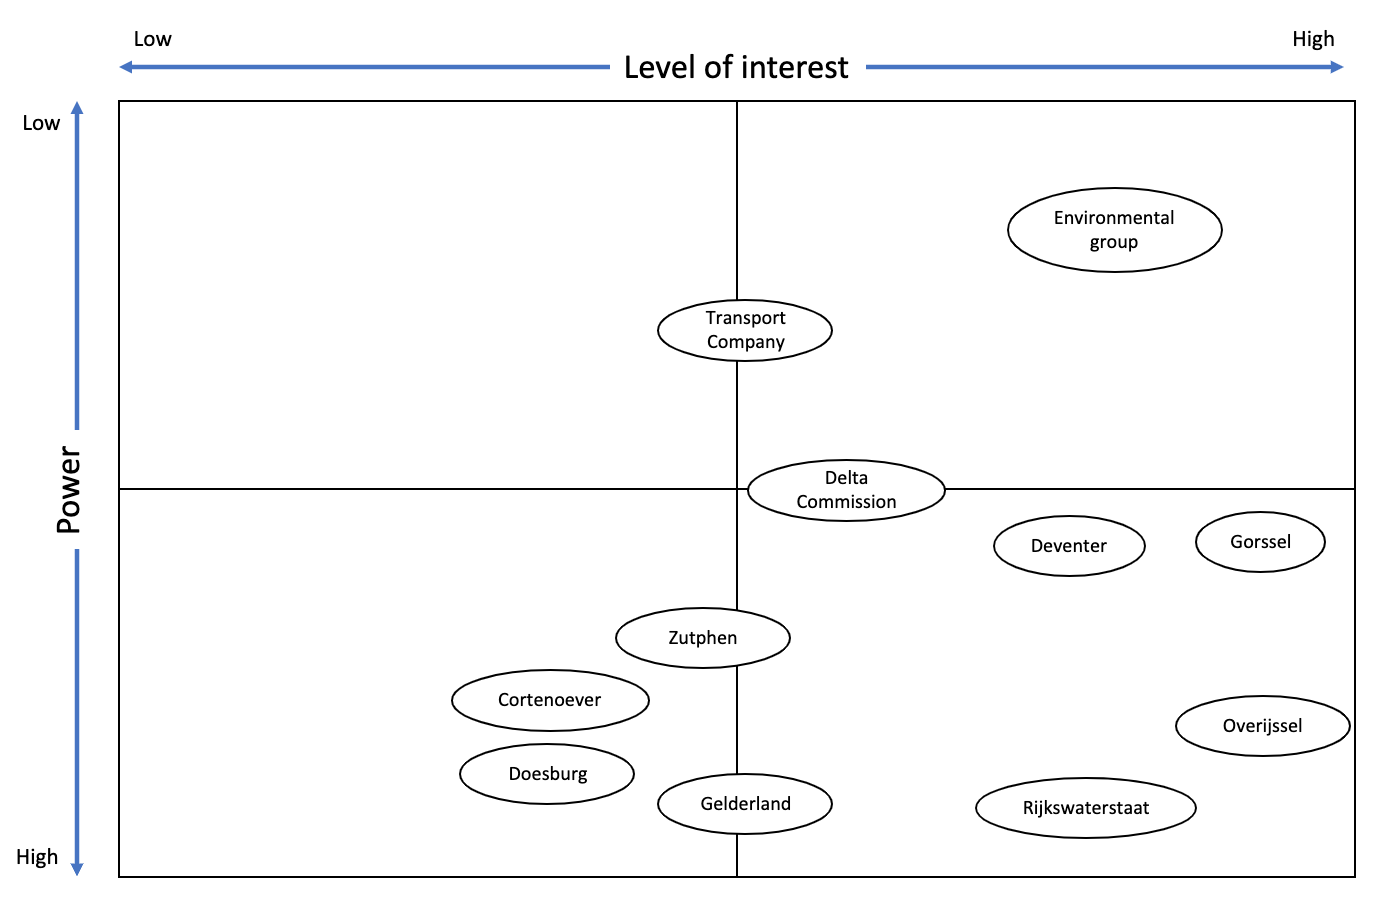
\includegraphics[width=0.7\textwidth]{report/figures/PI grid.png}
    \caption{Initial Power Interest Grid}
    \label{fig:pi-grid}
\end{figure}


%It is important to show an awareness of the political arena within which your problem owner is operating. It is also possible to entertain more than one problem formulation.
%Three problem formulations were developed in the EMA Workbench, to reflect the positions and objectives of Gorssel, and the other two actors.

% Explicit framing of problem from multiple relevant perspective (i.e. rival framings)
% Rival framings considered include Overijssel and Deventer, as these were seen as being the most consequential to our group.
% Rival actors
    % Deventer: utilitarian framing, more people in city! Hence city actually > farmers
    % Overijssel: framing itself as facilitator between Gorssel & Deventer, can take more passive role: city farmers battle it out, we implement whatever you figure out.
% a) Actor Analysis
As can be deduced, the Room for the River Project is complex multi-actor initiative and therefore objectives between the stakeholders will not always align. Knowing that Rijkswaterstaat, Deventer and Overijssel are actors with a high interest and high power in the issue means that they are the ones to watch out for. Knowing this, we will study the actors' objectives as it is important to keep in mind potential rival actors and conceptualise possible arguments and framings they can/will use to counter the aims of the client, Gorssel. All involved actors and their objectives for the RfR decision arena are listed in Table \ref{t:actortable}.

\begin{table}[h!]
\caption{-}
\begin{tabular}{p{0.2\textwidth}p{0.3\textwidth}p{0.4\textwidth}}
\hline 
Actor & Interest & Objective \\ \hline
Rijkswaterstaat         & Flood risk mitigation, Maintenance of water infrastructure & designing flood protection with widespread support \\ 
Delta Commission        & Long-term Flood Risk Mitigation & implementing effective and robust flood protection projects \\
Transport Company       & Efficient Road Network & ensuring accessibility/connectivity between various cities \\
Env. Protec. Gr.        & Environmental protection & minimising land use change in protected areas due to RfR \\
Gelderland              & Flood risk mitigation, Approval of residents & ensuring equitable time/cost distribution among provinces and municipalities \\
Cortenoever/Doesburg    & Livability for residents & minimising land use change \\
Overijssel              & Flood risk mitigation, Approval of Residents & ensuring equitable time/cost distribution among provinces and municipalities \\
Deventer                & Livability for residents, Aesthetic quality of the city & improving flood security to residents, minimising land use change \\
Gorssel                & Livelihood of resident farmers & protecting farmland, minimising profit loss \\
\end{tabular}
\label{t:actortable}
\end{table}

\bigskip 
% b) Justification of Rival Actors
Considering the power interest matrix as shown in figure \ref{fig:pi-grid} as well as relations between actors, Deventer and Overijssel are chosen as rival actors to explore alternate problem formulations. Since both Gorssel and Deventer are both administered by the Overijssel provincial government, there is the greatest chance of having conflicting goals and objectives regarding land use change, possibly resulting in negative outcomes for the client. At the same time these two actors also present opportunity of finding common ground and forming coalitions, to support one another at the negotiation table with other provinces, like Gelderland, and to ensure that a mutually beneficial proposal is drafted by the Rijkswaterstaat. The actions of other cities (those in Gelderland province) have been converted to uncertainties in the model.

\bigskip 

% c) Political Reflection (Framing)
Opposing stances from rival actors will be accompanied by an alternate framing of the problem. This framing can then be used to justify their actions. The city of Deventer, a much larger and older municipality of roughly 100 000 inhabitants, will be able to argue from a utilitarian point of view that it should carry greater weight in decision-making. Due to its cultural heritage it can also argue that land encroachment would be far more invasive compared to relocating several farms from the community of Gorssel. 

Overijssel, being the next level administrative body above Gorssel and Deventer, will have greater influence on which flood mitigation measures are implemented in higher level policy negotiations. As a provincial government, Overijssel is required to find some sort of balance of impacts between urban and rural communities. Due to Deventer's larger economic importance it may use similar framing to legitimise claims for needing to implement certain measures over others. Regional policy-makers can also obscure discourse using ill-defined neologisms, for example hybrid concepts such as "nature development" and "spatial quality" \parencite{warner_implementing_2011}. These empty signifiers combine environmental with economic values, to appear holistic and fair. Yet, these frames do not address social and economic concerns of Gorssel's population and fail to address increasing divide between urban and rural populations. These views can thus still be challenged and refine definition to specifically address these problems.

\smallskip  

The prioritised objectives for the Deventer-perspective problem formulation are:
\begin{itemize}
    \item Minimise Expected Annual Damage for Deventer: This objective reflects Gorssel's desire to generally minimise flood risk, while also reflecting effects of damage to farms and other property
    \item Minimise Expected Number of Deaths for Deventer: This objective reflects Gorssel's desire to generally minimse flood risk.
    \item Minimise Total Costs: This objective reflects the desire to reduce the cost impact of flood mitigation measures taken across the entire IJssel River system. Total costs for all actors was considered relevant given the requirement of cost sharing for flood mitigation activities across the region.
\end{itemize}
For Deventer, the policy lever for dike heightening in Deventer is switched off in the model, to reflect Deventer's hard constraint around encroachment of sites of cultural and historical significance in the city centre.

The prioritised objectives for the Overijssel-perspective problem formulation are:
\begin{itemize}
    \item Minimise Expected Annual Damage for Gorssel and Deventer: This objective reflects Gorssel's desire to generally minimise flood risk, while also reflecting effects of damage to farms and other property
    \item Minimise Expected Number of Deaths for Gorssel and Deventer: This objective reflects Gorssel's desire to generally minimse flood risk.
    \item Minimise Total Costs: This objective reflects the desire to reduce the cost impact of flood mitigation measures taken across the entire IJssel River system. Total costs for all actors was considered relevant given the requirement of cost sharing for flood mitigation activities across the region.
\end{itemize}

As is done for Gorssel, the actions of other actors in Gelderland province are treated as uncertainties in both Deventer's and Overijssel's problem formulations.

% \textcolor{red}{Should we include something in the description of Gorssel as a client to say that they have a low risk tolerance or something like that to justify choice of RDM over DAPP?}